%! Author = Son Trinh
%! Date = 10/13/2022

\begin{frame}{Gaussian Processes (GP) -- method summary}

\maketag{regression} \maketag{classification} \maketag{nonparametric} \maketag{probabilistic}

\medskip

\highlight{General idea}
\begin{itemize}
  \item GPs model a distribution over potential functions $\bm{f}$ that fit the observed data
  \item \textbf{Assumptions}:
  \begin{itemize}
     \item $n$-observations follow a $n$-dimensional Normal distribution
     \item The closer observations are, the higher they are correlated
  \end{itemize}
  \item A \textbf{kernel} function $k(\xi, \xv^{(j)})$ quantifies the similarity between two observations and induced the coviariance matrix of the distribution. 
  \item \textbf{Predict} via the maximum a-posteriori (MAP) estimate.
\end{itemize}

\medskip

\highlight{Hypothesis space} ~~
$\Hspace = \left\{ \bm{f} = \left[f\left(\xi[1]\right), \dots, f\left(\xi[n]\right)\right] \sim \mathcal{N}\left(\bm{m}, \bm{K}\right) ~|~ \bm{m} \in \R^n, \bm{K} \in \R^{n\times n} \right\}$

\medskip

\begin{minipage}[b]{0.5\textwidth}
  % FIGURE SOURCE: https://docs.google.com/presentation/d/1xodP6ayu1Gay6mMKgzVWYEFmSoeG5kNuqsaTkFFmd78  /edit
  \centering
  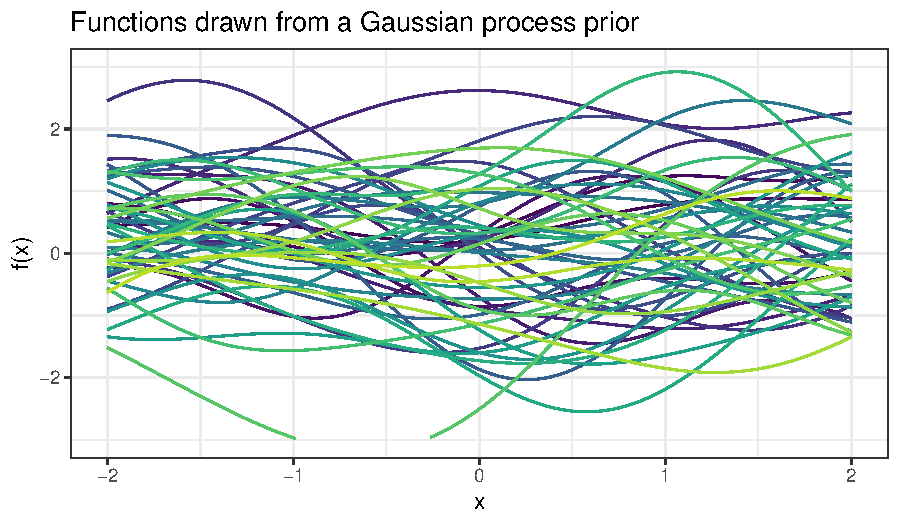
\includegraphics[width=0.7\textwidth]{figure/gp-prior} \\
\end{minipage}%
\begin{minipage}[b]{0.5\textwidth}
\centering
  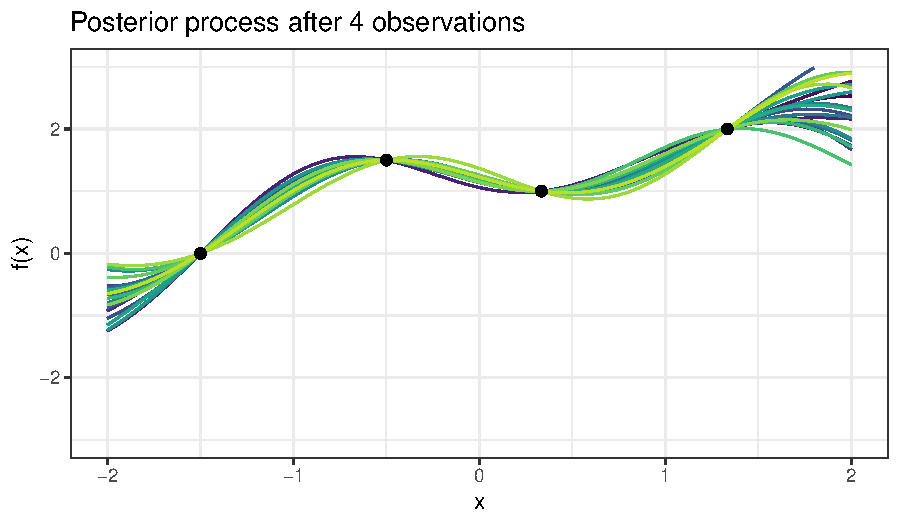
\includegraphics[width=0.7\textwidth]{figure/gp-posterior}
\end{minipage}

\end{frame}

% ------------------------------------------------------------------------------

\begin{frame}{Gaussian Processes (GP) -- method summary}
    
    \highlight{Empirical risk}
    \begin{itemize}
        \item The risk is estimated by using the posterior of a conditional Normal distribution
        \item Most kernels have \textbf{length scale parameters} that need to be estimated
    \end{itemize}
    \highlight{Optimization}
    \begin{itemize}
        \item The kernel parameters can be learned using \textbf{maximum likelihood} estimation
        \item This requires inverting the $n\times n$ -covariance matrix
    \end{itemize}
    \highlight{Hyperparameters}
    \begin{itemize}
        \item The most important hyperparameter is the choice of the kernel function $k(\xi, \xv^{(j)})$
        \item Common kernel choices for \textit{"standard"} data are:
        \begin{itemize}
            \item Linear or polyomial
            \item Squared-exponential (infinitely differentiable)
            \item Matérn (further generalization of the Squared-exponential kernel)
        \end{itemize}
        \item Special kernels for all kind of data situation exist, e.g., a Exp-Sine-Squared kernel for periodic data
        \item Kernels can be composed by multiplying or addition to create more expressive structures
    \end{itemize}
    
\end{frame}

% ------------------------------------------------------------------------------

\begin{frame}{GP -- Implementation \& Practical hints}

\highlight{Scalable GPs for larger data}
\begin{itemize}
	\item Low-rank approximations of the covariance by using only a representative subset of \textbf{inducing points}
	\item Using a kernel that creates a sparse coviariance matrix
\end{itemize}

\medskip

\highlight{Noisy GPs}
\begin{itemize}
    \item Having an interpolator might not be suitable if the data is noisy
    \item A noisy GP adds a \textbf{nugget} effect to the kernel $k(\xi, \xv^{(j)}) + \sigma\delta_{ij}$, creating a Gaussian process regression model
\end{itemize}

\medskip

\highlight{Implementation}

\begin{itemize}
  \item \textbf{R:} \texttt{mlr3} learners \texttt{LearnerClassifGausspr} /
    \texttt{LearnerRegrGausspr}, calling \texttt{kernlab::gausspr()}
  \item \textbf{Python:} \texttt{GaussianProcessClassifier} /
  \texttt{GaussianProcessRegressor} from package \texttt{scikit-learn}, \texttt{gpytorch} for a modular, scalable, efficient and GPU accelerated implementation built on \texttt{torch}
\end{itemize}

\end{frame}

\begin{frame}{Gaussian Processes (GP) -- Pros \& Cons}

\begin{columns}[onlytextwidth]
  \begin{column}{0.5\textwidth}
    \highlight{Advantages}
    \footnotesize
    \begin{itemize}
      \positem GPs allow to \textbf{quantify prediction uncertainty} induced by both intrinsic noise in the problem and errors in the parameter estimation process
      \positem A GP is a function \textbf{interpolator} and will predict the exact value of a training point
      \positem The choice of kernel function allows considerable flexibility for problem specific characteristics
      \positem Automatic relevance determination (ARD) determines the importance of features
      %\positem GP is \textbf{non-parametric} and can model virtually any functions of observations
    \end{itemize}
  \end{column}
  \begin{column}{0.5\textwidth}
    \highlight{Disadvantages}
    \footnotesize
    \begin{itemize}
      \negitem GPs are \textbf{not sparse}, i.e., they require the full training data for prediction
      \negitem GP training requires $\mathcal{O}(n^3)$, i.e., it scales cubically in the number of observations
      \negitem GPs cannot handle categorical features.
      \negitem GPs are \textbf{not particularly easy to understand} conceptually
    \end{itemize}
  \end{column}
\end{columns}

\end{frame}
